\documentclass[
	classe=$1^{ere}$STI2D
]{coursclass}

\usepackage{annotate-equations}
\usepackage{xfp}

\title{Cours Chapitre 2}
\author{Généralités sur les fonctions}
\date{}

\begin{document}

\begin{exemple}
	La fonction $f(x) = 2x$ a pour graphe
	\begin{center}
		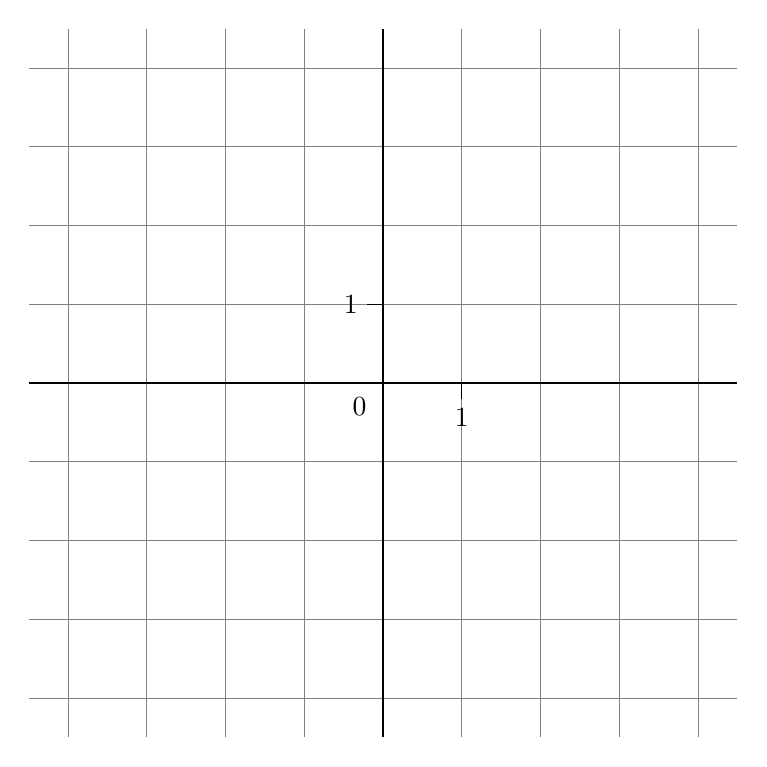
\begin{tikzpicture}
			\draw[thin,gray] (-4.5,-4.5) grid (4.5,4.5);
			\draw[thick,\myArrow] (-4.5,0) -- (4.5,0);
			\draw[thick,\myArrow] (0,-4.5) -- (0,4.5);
			\draw (1,0) -- ++(0,-0.2) node[below] {$1$};
			\draw (0,1) -- ++(-0.2,0) node[left] {$1$};
			\node at (-0.3,-0.3) {$0$};

			\ifdefined\makeCorrection
				\draw[orange,ultra thick,variable=\x,domain=-2.25:2.25] plot({\x},{2*\x}) node[right] {$𝒞_f$};
			\fi
		\end{tikzpicture}
	\end{center}

	La fonction $g(x) = -\dfrac{x}{2} + 1$ a pour graphe
	\begin{center}
		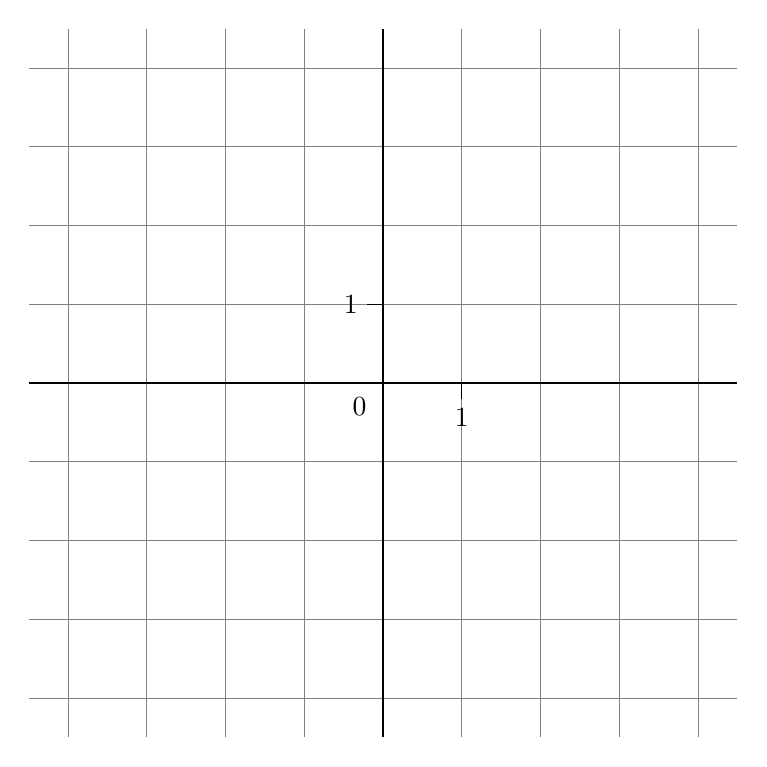
\begin{tikzpicture}
			\draw[thin,gray] (-4.5,-4.5) grid (4.5,4.5);
			\draw[thick,\myArrow] (-4.5,0) -- (4.5,0);
			\draw[thick,\myArrow] (0,-4.5) -- (0,4.5);
			\draw (1,0) -- ++(0,-0.2) node[below] {$1$};
			\draw (0,1) -- ++(-0.2,0) node[left] {$1$};
			\node at (-0.3,-0.3) {$0$};

			\ifdefined\makeCorrection
				\draw[orange,ultra thick,variable=\x,domain=-4.5:4.5] plot({\x},{-\x/2 + 1}) node[right] {$𝒞_g$};
			\fi
		\end{tikzpicture}
	\end{center}
\end{exemple}

\end{document}